\documentclass[11pt]{article}
\usepackage[utf8]{inputenc}
\usepackage[T1]{fontenc}

\usepackage[margin=2.5cm]{geometry}
\usepackage{amsmath,amssymb,amsthm}
\usepackage{tikz}
\usepackage{pgfplots}
\pgfplotsset{compat=1.17}
\usetikzlibrary{arrows.meta}
\usepgfplotslibrary{fillbetween}
\usepackage[most]{tcolorbox}

\newtcolorbox{obsbox}[1]{colback=blue!4,colframe=blue!50!black,fonttitle=\bfseries,title=#1}

\newtheorem{proposicion}{Proposición}
\renewcommand{\proofname}{Demostración}
\renewcommand{\figurename}{Figura}

\title{Conos tangente y linealizado en un ejemplo\\donde fallan las condiciones de KKT}
\date{20 de octubre de 2026}

\begin{document}
\maketitle

\section{Problema}

\begin{obsbox}{Problema}
\[
\min_{x\in\mathbb{R}^2}\; f(x)=x_1
\quad\text{s.a.}\quad
g_1(x)=-x_2\le 0,\qquad g_2(x)=x_2-x_1^3\le 0 .
\]
Punto candidato: $\bar x=(0,0)^T$.
\end{obsbox}

\paragraph{Conjunto factible.}
\[
C=\{x\in\mathbb{R}^2:\ 0\le x_2\le x_1^3\}.
\]
Como $0\le x_2\le x_1^3$ implica $x_1^3\ge 0$, todo punto factible cumple $x_1\ge 0$. Luego $f(x)=x_1\ge 0=f(\bar x)$ en $C$, y $\bar x$ es el mínimo global. El conjunto $C$ es una cúspide delgada entre el eje $x_1\ge 0$ y la curva $x_2=x_1^3$ (Figura~\ref{fig:cusp}).

\paragraph{Gradientes en $\bar x$.}
Ambas restricciones son activas: $g_1(\bar x)=g_2(\bar x)=0$, es decir, $\mathcal A(\bar x)=\{1,2\}$.
\[
\nabla f(\bar x)=\begin{pmatrix}1\\0\end{pmatrix},\qquad
\nabla g_1(\bar x)=\begin{pmatrix}0\\-1\end{pmatrix},\qquad
\nabla g_2(\bar x)=\begin{pmatrix}-3\bar x_1^2\\ 1\end{pmatrix}=\begin{pmatrix}0\\1\end{pmatrix}.
\]

\section{Cono linealizado}

\begin{proposicion}
$L(\bar x)=\{d\in\mathbb{R}^2:\ d_2=0\}=\{(d_1,0)^T:\ d_1\in\mathbb{R}\}$.
\end{proposicion}

\begin{proof}
Por definición, $L(\bar x)=\{d:\ \nabla g_i(\bar x)^Td\le 0,\ i\in\mathcal A(\bar x)\}$. Entonces
\[
\nabla g_1(\bar x)^Td=-d_2\le 0
\quad\text{y}\quad
\nabla g_2(\bar x)^Td=d_2\le 0,
\]
de donde $d_2=0$, mientras que $d_1$ queda libre.
\end{proof}

\section{Cono tangente}

\paragraph{Definición (cono tangente de Bouligand).}
$d\in T(\bar x,C)$ si existen una sucesión de direcciones $d_k\to d$ y una sucesión de escalares $t_k\to 0^+$ tales que
\[
\bar x+t_k d_k\in C\qquad\text{para todo }k\in\mathbb{N}.
\]
Es decir, $d$ es tangente si, perturbando ligeramente la dirección ($d_k$ en lugar de $d$), se puede dar pasos cada vez más cortos ($t_k$) desde $\bar x$ sin salir de $C$.

\paragraph{Por qué aparecen límites.} La definición no da una fórmula para $T(\bar x,C)$, sino la existencia de sucesiones. Para decidir qué direcciones pertenecen al cono hay dos tareas:
\begin{itemize}
  \item[($\subseteq$)] Suponer que las sucesiones existen, escribir la condición $\bar x+t_kd_k\in C$ como desigualdades en $d_k$ y $t_k$, y pasar al límite $k\to\infty$. Las desigualdades que sobreviven son condiciones necesarias sobre $d$.
  \item[($\supseteq$)] Para cada $d$ candidata, construir explícitamente $d_k$ y $t_k$ que cumplan la definición.
\end{itemize}
Para evitar confusión con potencias, escribimos las componentes de $d_k$ como $d_k=(u_k,v_k)^T$.

\begin{proposicion}
$T(\bar x,C)=\{(d_1,0)^T:\ d_1\ge 0\}$.
\end{proposicion}

\begin{proof}
($\subseteq$) Sea $d=(d_1,d_2)^T\in T(\bar x,C)$. Existen $d_k=(u_k,v_k)^T\to d$ y $t_k\to 0^+$ con $\bar x+t_kd_k=(t_ku_k,\,t_kv_k)^T\in C$, es decir,
\[
0\le t_kv_k\le (t_ku_k)^3=t_k^3u_k^3\qquad\text{para todo }k.
\]
Dividiendo por $t_k>0$,
\[
0\le v_k\le t_k^2\,u_k^3\qquad\text{para todo }k. \tag{$\ast$}
\]
\begin{itemize}
  \item De $(\ast)$, $t_k^2u_k^3\ge 0$ y $t_k^2>0$, luego $u_k\ge 0$. Como $u_k\to d_1$, se obtiene $d_1\ge 0$.
  \item Pasando al límite en $(\ast)$: $v_k\to d_2$ y $t_k^2u_k^3\to 0\cdot d_1^3=0$ (pues $t_k\to 0$ y $u_k\to d_1$ es acotada). Por lo tanto $0\le d_2\le 0$, es decir, $d_2=0$.
\end{itemize}
Así $d_1\ge 0$ y $d_2=0$.

($\supseteq$) Sea $d=(d_1,0)^T$ con $d_1\ge 0$. Tomemos la sucesión constante $d_k=d$ y $t_k=1/k\to 0^+$. Entonces
\[
\bar x+t_kd_k=\left(\tfrac{d_1}{k},\,0\right)^T\in C,
\]
pues $0\le 0\le \left(\tfrac{d_1}{k}\right)^3$. Luego $d\in T(\bar x,C)$.
\end{proof}

\paragraph{Ejemplo: por qué $(-1,0)^T\notin T(\bar x,C)$.} Si existieran $d_k=(u_k,v_k)^T\to(-1,0)^T$ y $t_k\to 0^+$ con $\bar x+t_kd_k\in C$, entonces $u_k<0$ para $k$ grande, lo que contradice $u_k\ge 0$ obtenido de $(\ast)$. Geométricamente, cualquier paso desde $\bar x$ hacia $x_1<0$ sale de $C$, por pequeño que sea.

\begin{figure}[h]
\centering
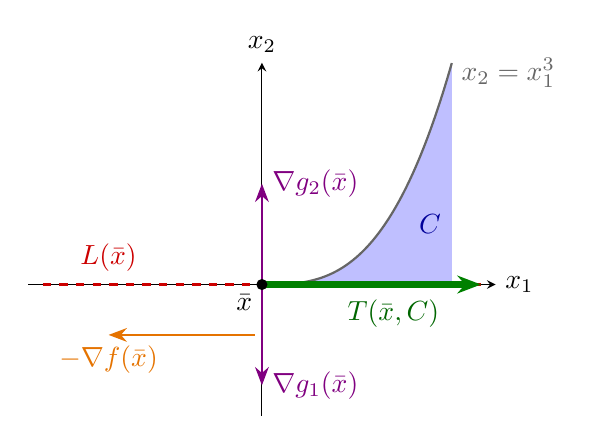
\begin{tikzpicture}
\begin{axis}[
  width=0.62\textwidth, height=0.5\textwidth,
  axis lines=middle, xmin=-1.6, xmax=1.6, ymin=-1.3, ymax=2.2,
  xlabel={$x_1$}, ylabel={$x_2$},
  xtick=\empty, ytick=\empty, clip=false,
  every axis x label/.style={at={(ticklabel* cs:1)},anchor=west},
  every axis y label/.style={at={(ticklabel* cs:1)},anchor=south},
]
  % feasible set C
  \addplot[name path=cubic, domain=0:1.3, samples=80, thick, black!60] {x^3};
  \addplot[name path=axis0, domain=0:1.3, draw=none] {0};
  \addplot[fill=blue!25, draw=none] fill between[of=cubic and axis0];
  \node[blue!60!black] at (axis cs:1.15,0.6) {$C$};
  \node[black!60, anchor=west] at (axis cs:1.3,2.1) {$x_2=x_1^3$};

  % linearized cone L: the whole x1-axis
  \draw[red!80!black, line width=1.2pt, dashed] (axis cs:-1.5,0) -- (axis cs:1.5,0);
  \node[red!80!black, anchor=south] at (axis cs:-1.05,0.03) {$L(\bar x)$};

  % tangent cone T: ray x1>=0
  \draw[green!50!black, line width=2.4pt, -{Stealth[length=3mm]}] (axis cs:0,0) -- (axis cs:1.5,0);
  \node[green!40!black, anchor=north] at (axis cs:0.9,-0.05) {$T(\bar x,C)$};

  % gradients
  \draw[-{Stealth}, thick, violet] (axis cs:0,0) -- (axis cs:0,-1) node[anchor=west] {$\nabla g_1(\bar x)$};
  \draw[-{Stealth}, thick, violet] (axis cs:0,0) -- (axis cs:0,1) node[anchor=west] {$\nabla g_2(\bar x)$};
  \draw[-{Stealth}, thick, orange!90!black] (axis cs:-0.05,-0.5) -- (axis cs:-1.05,-0.5)
      node[anchor=north] {$-\nabla f(\bar x)$};

  \fill (axis cs:0,0) circle (2pt);
  \node[anchor=north east] at (axis cs:0,0) {$\bar x$};
\end{axis}
\end{tikzpicture}
\caption{Conjunto factible $C$ (sombreado), cono tangente $T(\bar x,C)$ (semirrecta verde) y cono linealizado $L(\bar x)$ (recta roja discontinua). La flecha naranja $-\nabla f(\bar x)=(-1,0)^T$ se dibuja desplazada verticalmente solo para que no se superponga con el eje.}
\label{fig:cusp}
\end{figure}

\section{Falla de las condiciones de calificación}

\begin{proposicion}
En $\bar x=(0,0)^T$ no se cumplen LICQ, MFCQ, Abadie ni Guignard.
\end{proposicion}

\begin{proof}
\textbf{LICQ.} Los gradientes activos $(0,-1)^T$ y $(0,1)^T$ son linealmente dependientes, ya que $\nabla g_1(\bar x)+\nabla g_2(\bar x)=0$.

\textbf{MFCQ.} Haría falta $d$ con $\nabla g_1(\bar x)^Td=-d_2<0$ y $\nabla g_2(\bar x)^Td=d_2<0$, es decir, $d_2>0$ y $d_2<0$ a la vez, lo cual es imposible.

\textbf{Abadie} ($T(\bar x,C)=L(\bar x)$). Se tiene $T(\bar x,C)\subsetneq L(\bar x)$. Por ejemplo, $d=(-1,0)^T\in L(\bar x)$, pero $d\notin T(\bar x,C)$ porque $d_1<0$.

\textbf{Guignard} ($T(\bar x,C)^\circ=L(\bar x)^\circ$). Calculamos los polares:
\[
T(\bar x,C)^\circ=\{v:\ v_1d_1\le 0\ \ \forall d_1\ge 0\}=\{v\in\mathbb{R}^2:\ v_1\le 0\},
\]
\[
L(\bar x)^\circ=\{v:\ v_1d_1\le 0\ \ \forall d_1\in\mathbb{R}\}=\{v\in\mathbb{R}^2:\ v_1=0\}.
\]
Como $(-1,0)^T\in T(\bar x,C)^\circ\setminus L(\bar x)^\circ$, los polares son distintos.
\end{proof}

\section{Conexión con la ausencia de multiplicadores}

Por el lema de Farkas, $L(\bar x)^\circ=\operatorname{cone}\{\nabla g_1(\bar x),\nabla g_2(\bar x)\}=\{(0,v_2)^T:\ v_2\in\mathbb{R}\}$, y las condiciones de KKT equivalen a
\[
-\nabla f(\bar x)\in L(\bar x)^\circ .
\]
Por otro lado, la condición geométrica de optimalidad sí se cumple: para todo $d\in T(\bar x,C)$,
\[
\nabla f(\bar x)^Td=d_1\ge 0,
\quad\text{es decir,}\quad
-\nabla f(\bar x)\in T(\bar x,C)^\circ .
\]
Pero $-\nabla f(\bar x)=(-1,0)^T\notin L(\bar x)^\circ$, porque su primera componente no es cero. Esa es exactamente la contradicción $1=0$ de la ecuación de KKT:
\[
(1,0)^T+\lambda_1(0,-1)^T+\lambda_2(0,1)^T=(0,0)^T .
\]

\begin{obsbox}{Conclusión}
\[
T(\bar x,C)=\{(d_1,0):\ d_1\ge 0\}\ \subsetneq\ L(\bar x)=\{(d_1,0):\ d_1\in\mathbb{R}\}.
\]
La linealización ``ve'' la dirección $(-1,0)$, que no es factible en la cúspide. En consecuencia $T^\circ\supsetneq L^\circ$ y $-\nabla f(\bar x)$ cae en la diferencia: $\bar x$ es óptimo, pero no admite multiplicadores de KKT.
\end{obsbox}

\end{document}
